\section{Arbitrary Data Injection}\label{sec:attack}

% NB: in the case of EOS, we think the only real difference between the downlinks DB and TDRSS is bit rate, from the space shuttle report

% Structure:
%
% Existing software exists (e.g. within IPOPP) to decode satellite signals
% However, no real software exists to encode signals
%
% Prerequisites:
% * Wireless communications packet structure and standards
% * IPOPP pipeline processing stages


The attacker fundamentally needs to overshadow the radio wave with a signal that decodes to the one that they want to inject.
Their aim is the delivery of arbitrary bytes, which will either violate the packet protocol to attempt to exploit a processing step, or cause problems in a satellite-derived dataset.
As a case study, we consider specifically the protocols used in the MODIS downlink of Terra and Aqua, due to the availability of documentation, their representative usage of standard space network layer protocols, and their broad usage in many critical satellite-derived datasets.
We consider how the attacker generates these bytes, the requirements to successfully overshadow the radio wave, and the broader effects of such an attack in Section \ref{sec:evaluation}.

In order to successfully inject bytes, the attacker must provide data that is parsed correctly by the relevant processing steps.
Doing this requires knowledge of the expected packet structure, alongside the processing stages in the pipeline.

\subsection{Terra and Aqua wireless communications specifications} % TODO: different title?

Terra and Aqua communicate on a number of different radio channels and downlink housekeeping, telemetry, and scientific data. \textbf{Are these all the unique ones?}
The satellites themselves can be in one of a number of operational modes, during which they send different information through the available channels. \textbf{TODO: cite SPACE GROUND AQUA document} % TODO: maybe talk about how you can find out more information about this in the appendix?
During nominal operation the satellite is in Direct Broadcast mode, in which the current MODIS sensor data is continuously downlinked.
The data is also buffered for high data rate downlink when the satellite passes over Polar Ground Stations or near its TDRSS relay.

Since the buffer is packed with the same bytes as the Direct Broadcast signal, the format of the data is identical for all modes of broadcast.
We therefore focus on the Direct Broadcast mode without loss of generality.

%To broadcast to the Polar Ground Stations therefore requires a temporary shift out of Direct Broadcast Mode.
%The schedule for direct broadcast can be found for Terra~\cite{terraSchedule} and Aqua~\cite{aquaSchedule} at the HTTP file archive for the Goddard Space Flight Center.

% TODO: describe the structure of each CADU and how the relevant fields e.g. IDs are used
Since each instrument onboard the satellite needs to downlink data simultaneously, the scientific data is sent in a packets to the Formatter/Multiplexer Unit (FMU).
The FMU encapsulates the instrument packets within CCSDS Space Packet Protocol (SPP) packets which contain an Application ID to support demultiplexing per instrument.
The SPP packets are then packed into a custom, unencrypted data link protocol known as the \textit{Channel Access Data Unit}, or CADU.
Finally, the CADUs are modulated onto a radio wave either immediately in the case of Direct Broadcast, or after a short delay for bulk transmission.

\subsection{MODIS downlink decoding pipeline}

On the ground, the signal is received by a tracking satellite antenna and passes through multiple different processing stages to firstly decode the wave into bits, then align the bytes, and finally interpret the data to form satellite-derived datasets.

The data is generally presented to the first software decoding stage as a stream of bits straight from a hardware demodulator component, which therefore presents the first opportunity to exploit a packet decoding stage.

These bits must firstly be byte aligned and divided into CADUs, derandomised through Viterbi decoding depending on the satellite mode, and then error corrected according to the CADU checksum.
These stages are sometimes implemented by dedicated hardware or as a separate piece of software, such as Dartcom's \textit{Polar Orbital Ingester}~\cite{dartcomsystemsltdXBand2021,dartcomPOI}.
However, they can equivalently be handled by NASA's \textit{Real-time Software Telemetry Processing System} (RT-STPS).

In addition to the previous steps, RT-STPS demultiplexes the CADUs and outputs the data they contain, which are in this case SPP packets.
The demultiplexing acts as a basic sanity check, ensuring that each packet has a valid application ID and size.
Through checking at hardcoded bit offsets, RT-STPS also tries to check whether the contents of the CADUs have the correct Application ID.

The resulting data is known as Level 0 data, and contains the demultiplexed CCSDS packets.
The Level 0 data is processed through a pipeline of programs within the IPOPP distribution into subsequently higher levels, eventually resulting in the satellite-derived datasets described in \textbf{TODO: make this table of MODIS data usage}.

\subsubsection{Decoding the packet format}

The Level 0 data consists of SPP packets containing the MODIS instrument packets.
In a single decoding step, the raw sensor readings within the packet are unpacked into a heirarchical data format (HDF), alongside some metadata.

This decoding step is therefore the last chance for an attacker to exploit a processing stage through malformed packet headers.
It is also the point beyond which the satellite-derived datasets are produced, which can be potentially fooled through injecting false or modified data which still conforms to the packet specifications.

%TODO: rephrase this
However, the software is easily exploitable due to some engineering problems


Each program within IPOPP has a standard interface written in XML which describes its available functions and operations.
The XML is parsed by a Java application which runs the available functions through interpreting the available functions using the shell, which generally spawns another program to continue the processing.
Although the interface is common among all IPOPP programs, the programs themselves are very diverse in language and architecture.


The Level 0 data passes through two stages of the \textit{MODIS Level-1 Science Processing Algorithm} (MODISL1DB\_SPA), resulting in heirarchical data format (HDF) files geolocated to a subpixel accuracy.

The first stage, known as \texttt{l0tol1}, processes Level 0 SPP data into Level 1 HDFs, which contains restructured raw sensor samples alongside other metadata.
The second stage, known as \texttt{l1atob}, geolocates the HDFs to a subpixel accuracy using timing information from the data, the satellite's orbital parameters, and an accurate model of the Earth's surface.
The resulting data is considered to be at Level 1B.

Each of these stages relies upon \textit{OceanColor Science Software} (OCSSW)~\cite{ocssw}, written by the OceanColor Data team \textbf{TODO: check}, to perform the actual processing.
In particular, \textbf{TODO: list the tools for each stage} perform the tasks of extracting the data, and correcting corrupted data in the case of failure.
The OCSSW tools are written in C and Fortran, and were originally designed to be run as command line scripts.
They expect a parameter file at a particular relative path \textbf{TODO: check} which itself describes the location of the data to be processed and supplies options for processing it.

In order to automate processing and correcting the data, Python programs were written which construct the command line arguments and parameter files required for the OCSSW tools, and then invoke a shell to execute the tools.
These are designed to be higher-level tools for use in analysing and processing the data files on the command line, which don't require knowledge of the arcane OCSSW formats.

Within IPOPP, \texttt{l0tol1} and \texttt{l1atob} are themselves shell scripts which call these Python programs with certain arguments callable from the XML interface.
\textbf{TODO: fact check that l1atob is actually a shell script and not the Python directly}

\subsubsection{Creating satellite-derived datasets}

% TODO: link to and cite the software manuals and SPA descriptions of each of these
The geolocated Level 1B HDFs proceed into the next processing stage, the \textit{Level 2 MODIS Active Fire Product} (MOD14).
MOD14 identifies active fires from the MODIS data and outputs HDF and txt files considered to be at Level 2. \textbf{TODO: cite manual}

% TODO: describe the structure of MOD14

Through analysing





% TODO: describe granules, and how the raw data gets divided into them?
% TODO: describe the arcane naming convention of the datasets
%   Is this better left for evaluation?

% l0tol1 is distributed twice, there's no version control anywhere
% Reaching out over raw http to servers for data

software within \textit{IPOPP}

% Description of the construction of IPOPP algorithms


%TODO: add details of which things it requires

also demultiplexes the CADUs

After being downconverted and sampled,




\subsection{Encoding arbitrary bytes}

\subsection{Manipulating existing data}


\begin{figure*}
    \centering
    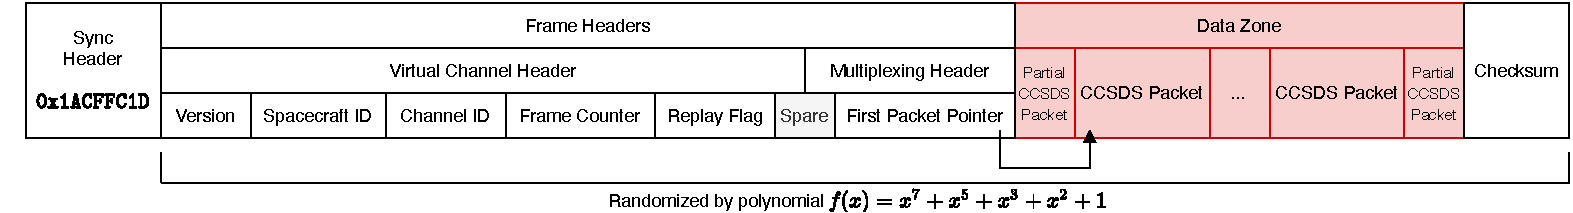
\includegraphics[width=\textwidth]{diagrams/cadu_diagram.pdf}
    \caption{Layout of data within a Channel Access Data Unit (CADU). Given correct headers, the section marked in red can contain arbitrary attacker-specified data. \textbf{TODO remove}}
    \label{fig:cadu_diagram}
\end{figure*}

\begin{figure}
    \centering
    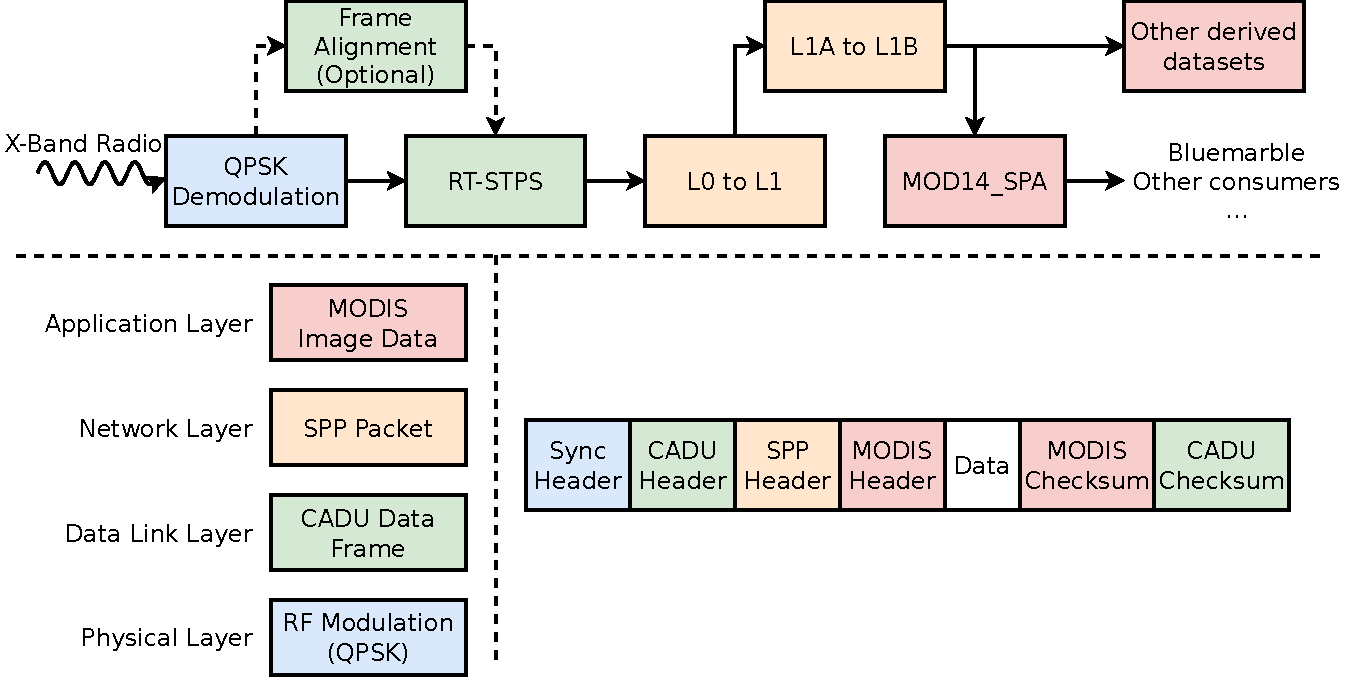
\includegraphics[width=\linewidth]{diagrams/attack_types.pdf}
    \caption{Illustration of the steps involved in processing MODIS image data and derived datasets, as well as the packet structure and layer within the network stack. \textbf{TODO edd rewrite?}}
    \label{fig:attack_types}
\end{figure}

% Wireless spec to go into attack, since it's specific to the MODIS use case
% \subsection{Wireless communications specifications}
% \textit{Discuss the protocols that are used, which will be correlated to later processing stages}

% In each of their downlink modes, \textit{Terra} and \textit{Aqua} communicate using frames modulated onto a carrier wave using quadrature phase shift keying (QPSK).
%In QPSK each symbol (pair of bits) is encoded by shifting the phase of the carrier wave
%In QPSK, symbols represent pairs of bits, and are encoded by shifting the phase of the carrier wave in one of four orientati.

%Information from each of the scientific instruments on the spacecraft is encoded according to the CCSDS packet standard, and are packed into frames known as Channel Access Data Units (CADUs).

%Each CADU is prefixed with a synchronisation header, enabling the receiver software to delimit the frames.
%The rest of the body is "randomised" through XORing with a fixed polynomial to prevent long sequences of the same symbol disrupting transfer.
%The full breakdown of the packet structure can be seen in Fig.~\ref{fig:cadu_diagram}.

%The finalised CADUs are transferred directly to the X-band antenna when in direct broadcast mode, and also to a solid state recorder for playback during the data dumps.


\subsection{Attack description}


Unfortunately the \textit{IPOPP} framework for processing EOS data is open to a variety of attacks through signal injection.
In each case, the attacker leverages different parts of the protocol to redirect the control flow of the program, either causing a denial of service, the leaking of sensitive data, or even arbitrary code execution.

Through the injection of standards-compliant frames, complete with synchronisation headers and checksums, the attacker can convince prior processing stages to decode and demultiplex an arbitrary byte sequence, delivering it as input to \textit{MODISL1DB\_SPA}.

The input to this algorithm is so-called \textit{Level 0} data, which is the body of a data frame with all communications artefacts, including synchronisation headers and checksums, removed.
Through the creation of a custom data frame, the attacker can encapsulate an arbitarary byte sequence which, when overshadowed over the existing signal, will result in the delivery of arbitrary bytes as the input to \textit{MODISL1DB\_SPA}.

We proceed to analyse several classes of attack made possible through this route, and enabled by insecure data handling practises.


\section{Exploiting downlink processing systems}

\subsubsection{Unprocessable malformed packets}

The software makes assumptions about the internal structure of the packets, which only hold for benign packets.
With the ability to inject arbitrary data, the attacker can craft packets to exploit oversights in the exception handling code for data parsing, and cause the program to crash.
Since the program processes packets in sets, a single malformed packet is sufficient to prevent the processing of the entire set.

Since the packet data is stored as a dataset for future processing, this attack also lets the attacker poison the dataset to make reprocessing of the entire set significantly harder.


\subsubsection{Latent arbitrary code execution}

In addition to near real-time data processing at the downlinks, past data is often reprocessed to take advantage of new processing alorithms, or to explore new results.
To support these use cases, the processing algorithms within MODISL1DB\_SPA are also available as command line tools, with adjustable configurations.

When run in SPA mode, the configuration used is always the same, which has resulted in a "golden path" through the execution of the program which is relatively secure.
However, by changing the initial configuration, a user could accidentally put the program into a mode which unsafely handles the input data.

Therefore, an attacker can poison the official datasets through the injection of packets, which cause no unsafe behaviour on first processing, but leverage vulnerabilities for arbitrary code execution when reprocessed under a different configuration.
These vulnerabilities have the potential to lie dormant in the official data sources as currently distributed by LAADS DAC, among other Direct Readout stations.

% TODO: go on to demonstrate the attack

\subsubsection{Reading unallocated memory}

Due to the design of the hardware on board the satellite, legitimate communications from the onboard instruments are guaranteed to hold to certain assumptions: for example, the packets are always of the same length, and the internal pointers between the packets are always aligned.

However, in this situation it becomes easy to let implicit assumptions about the structure of the data manifest themselves in the data processing.
Code for handling these exceptional cases is often less rigorously tested, because it generally doesn't occur in benign example cases.

However, by providing shorter packets than expected, with larger pointers than expected, we demonstrate how the attacker can take advantage of certain system components written in C to read off the end of the buffer into unallocated memory.
We demonstrate an execution pathway that would result in the resulting data being stored and uploaded to the public data archives, theoretically allowing the attacker to leak sensitive information from other processes within the memory of the computer.


\subsubsection{Exploiting bundled dependencies}

In order to make software distribution easier, and to create easily deployable systems that mostly "just work" when extracted into a certain location, the IPOPP algorithms generally come with many bundled dependencies in the source archive.
These files are compiled programs and libraries for the handling of input data, that are intended to work on specific architectures.

However, the practice of bundling libraries with software has long been considered bad from a security perspective, especially since the widespread use of package managers to resolve and install dependencies.
Doing so permits a similar ease of installation, but allows each library and program to be traced back to its dependency, independently updated, and uninstalled when no longer required.

Without a system for managing these dependencies, the system becomes incredibly brittle and hard to change; therefore, there are many dependencies currently present and depended upon that haven't been updated in nearly a decade.
Several of these dependencies have patchable security vulnerabilities for arbitrary code execution, that an attacker could take advantage of.

There are also a large number of dependencies that aren't used for any purpose and are just left around for legacy reasons.
Besides potentially being a risk for privilege escalation, the sheer number of redundant dependencies muddies the water and makes it difficult to discern which depencies need updating as a matter of urgency.

% \begin{itemize}
%     \item Strict separation of data handling code from core program control flow
%     \item Secure distribution and patching of dependencies
%     \item Robustness against configuration changes
% \end{itemize}
